% TeX'ing this file requires that you have AMS-LaTeX 2.0 installed
% as well as the rest of the prerequisites for REVTeX 4.0
%
% See the REVTeX 4 README file
% It also requires running BibTeX. The commands are as follows:
%
%  1)  latex apssamp.tex
%  2)  bibtex apssamp
%  3)  latex apssamp.tex
%  4)  latex apssamp.tex
%
\documentclass[prb,preprintnumbers,amsmath,amssymb, 11pt]{revtex4}
%\documentclass[preprint,showpacs,showkeys,preprintnumbers,amsmath,amssymb]{revtex4}

% Some other (several out of many) possibilities
%\documentclass[preprint,aps]{revtex4}
%\documentclass[aps, two column, amsmath,amssymb,floatfix]{revtex4}
%\documentclass[showkeys,showpacs,amsmath,amssymb,onecolumn,superscriptaddress,prl]{revtex4-1}% Physical Review B  
% \documentclass[aps,prl,reprint,showpacs,floatfix,superscriptaddress, onecolumn]{revtex4-2}

\usepackage{amsmath,amsthm,amssymb}
\usepackage{graphicx}% Include figure files
\usepackage{dcolumn}% Align table columns on decimal point
\usepackage{bm}% bold math
\usepackage{color}
\usepackage{epsfig}
\usepackage{multirow}
\usepackage{mathrsfs}
\usepackage{hyperref}
\usepackage{cleveref}
\usepackage{epstopdf}
\usepackage{subcaption}
\usepackage{autobreak}
\usepackage{tikz}
\usepackage{svg}

%Macros for mathematical notations

\newcommand{\V}[1]{\boldsymbol{#1}} %# vector
\newcommand{\M}[1]{\boldsymbol{#1}} %# matrix
\newcommand{\Set}[1]{\mathbb{#1}} %# set
\newcommand{\D}[1]{\Delta#1} %# \D{t} for time step size
\renewcommand{\d}[1]{\delta#1} %# \d{t} for small increment
\newcommand{\norm}[1]{\left\Vert #1\right\Vert } % norm
\newcommand{\abs}[1]{\left|#1\right|} %abs

\newcommand{\grad}{\M{\nabla}} %gradient
\newcommand{\av}[1]{\left\langle #1\right\rangle } %take average

\newcommand{\sM}[1]{\M{\mathcal{#1}}} %matrix in mathcal font
\newcommand{\dprime}{\prime\prime} % double prime
%\global\long\def\i{\iota}
%\renewcommand{\i}{\iota} %i for imaginary unit
%\renewcommand{\i}{\mathsf i} %i for imaginary unit
\newcommand{\follows}{\quad\Rightarrow\quad} %=>
\newcommand{\eqd}{\overset{d}{=}} %=^d
\newcommand{\spe}[1]{\mathscr{#1}}  %important quantities in mathscr font
\newcommand{\eps}{\epsilon}
\newcommand{\bra}[1]{\left\langle #1 \right|}
\newcommand{\ket}[1]{\left| #1 \right\rangle}
\newcommand{\braket}[2]{\left\langle #1 \middle| #2 \right\rangle}
\newcommand{\bracket}[3]{\left\langle #1 \middle| #2 \middle| #3 \right\rangle}

\newtheorem{theorem}{Theorem}[section]
\newtheorem{lemma}[theorem]{Lemma}
\newtheorem{definition}[theorem]{Definition}



\begin{document}
\preprint{Preprint}

\title{Bare interaction of mono-layer graphene $p_z$ orbital}
\author{}
% \date{}

\maketitle

\section{Bare interaction: monolayer graphene $p_z$ orbitals}

We evaluate the bare Coulomb matrix elements
\begin{equation}
  U_{abcd}=\int d\V r\,d\V r'\,\phi_a^*(\V r)\phi_b(\V r)\,\frac{1}{|\V r-\V r'|}\,\phi^*_c(\V r')\phi_d(\V r')
\end{equation}
on the carbon $p_z$ Wannier orbitals from Wannier90 (5$\times$5$\times$1 supercell, $150\times150\times192$ grid). 

Reference values used for comparison:
\begin{itemize}
  \item CoQui cRPA bare channels (Malte R\"osner, $k$-mesh $16\times16\times1$, $n_b{=}144$, $c{=}15$).
  \item Wehling \emph{et al.}, Phys.~Rev.~Lett.~\textbf{106}, 236805 (2011), Table~I (freestanding graphene, equilibrium lattice).
\end{itemize}

\begin{table}[h]
\centering
\caption{Bare $p_z$--$p_z$ Coulomb matrix elements for monolayer graphene, in eV. ``This work'' uses \texttt{source\_tol = volume\_tol = $10^{-3}$} on the raw Wannier90 XSF grid. Relative differences are quoted against the CoQui value.}
\label{tab:mlg_bare}
\begin{tabular}{lcccccc}
\hline\hline
Channel & Symbol & This work & CoQui (cRPA bare) & PRL 106, 236805 & $\Delta$ vs.\ CoQui \\
\hline
On-site                & $U_{00}$ (onsite)   & 16.400 & 17.434 & 17.0 & $-5.93\%$ \\
Nearest neighbor       & $U_{01}$ (NN)       &  8.529 &  8.840 &  8.5 & $-3.51\%$ \\
Hund's exchange (s.f.) & $J^{\mathrm{sf}}$   &  0.1175 & 0.1308 & --   & $-10.17\%$ \\
Hund's pair-hopping    & $J^{\mathrm{ph}}$   &  0.1175 & 0.1308 & --   & $-10.17\%$ \\
\hline\hline
\end{tabular}
\end{table}

The two Hund's channels agree numerically ($|J^{\mathrm{sf}}-J^{\mathrm{ph}}|<10^{-16}$), confirming the real-orbital identity $V_{abba}=V_{abab}$. 
% The residual underestimate relative to CoQui is consistent with under-resolution of the orbital cusp at the C nucleus on the $\sim$0.08~\AA{} XSF grid; a mirror-pad xy-tail diagnostic was inconclusive because the Wannier90 output already fills the 5$\times$5 supercell periodically. 
The difference with CoQui is likely because the CoQui cRPA run was under a periodic setup, which may have led to an overestimate of the bare interaction due to the periodic images.
Only the on-site and NN channels are reported here---$U_{02}$, $U_{03}$ require shifting the second orbital onto further-neighbor sublattice sites, which has not been done in this run.

\section{Tolerance convergence}

The TKM3D quadrature tolerances \texttt{source\_tol} and \texttt{volume\_tol} were swept jointly from~$10^{-3}$ to $10^{-5}$.

\begin{figure}[h]
\centering
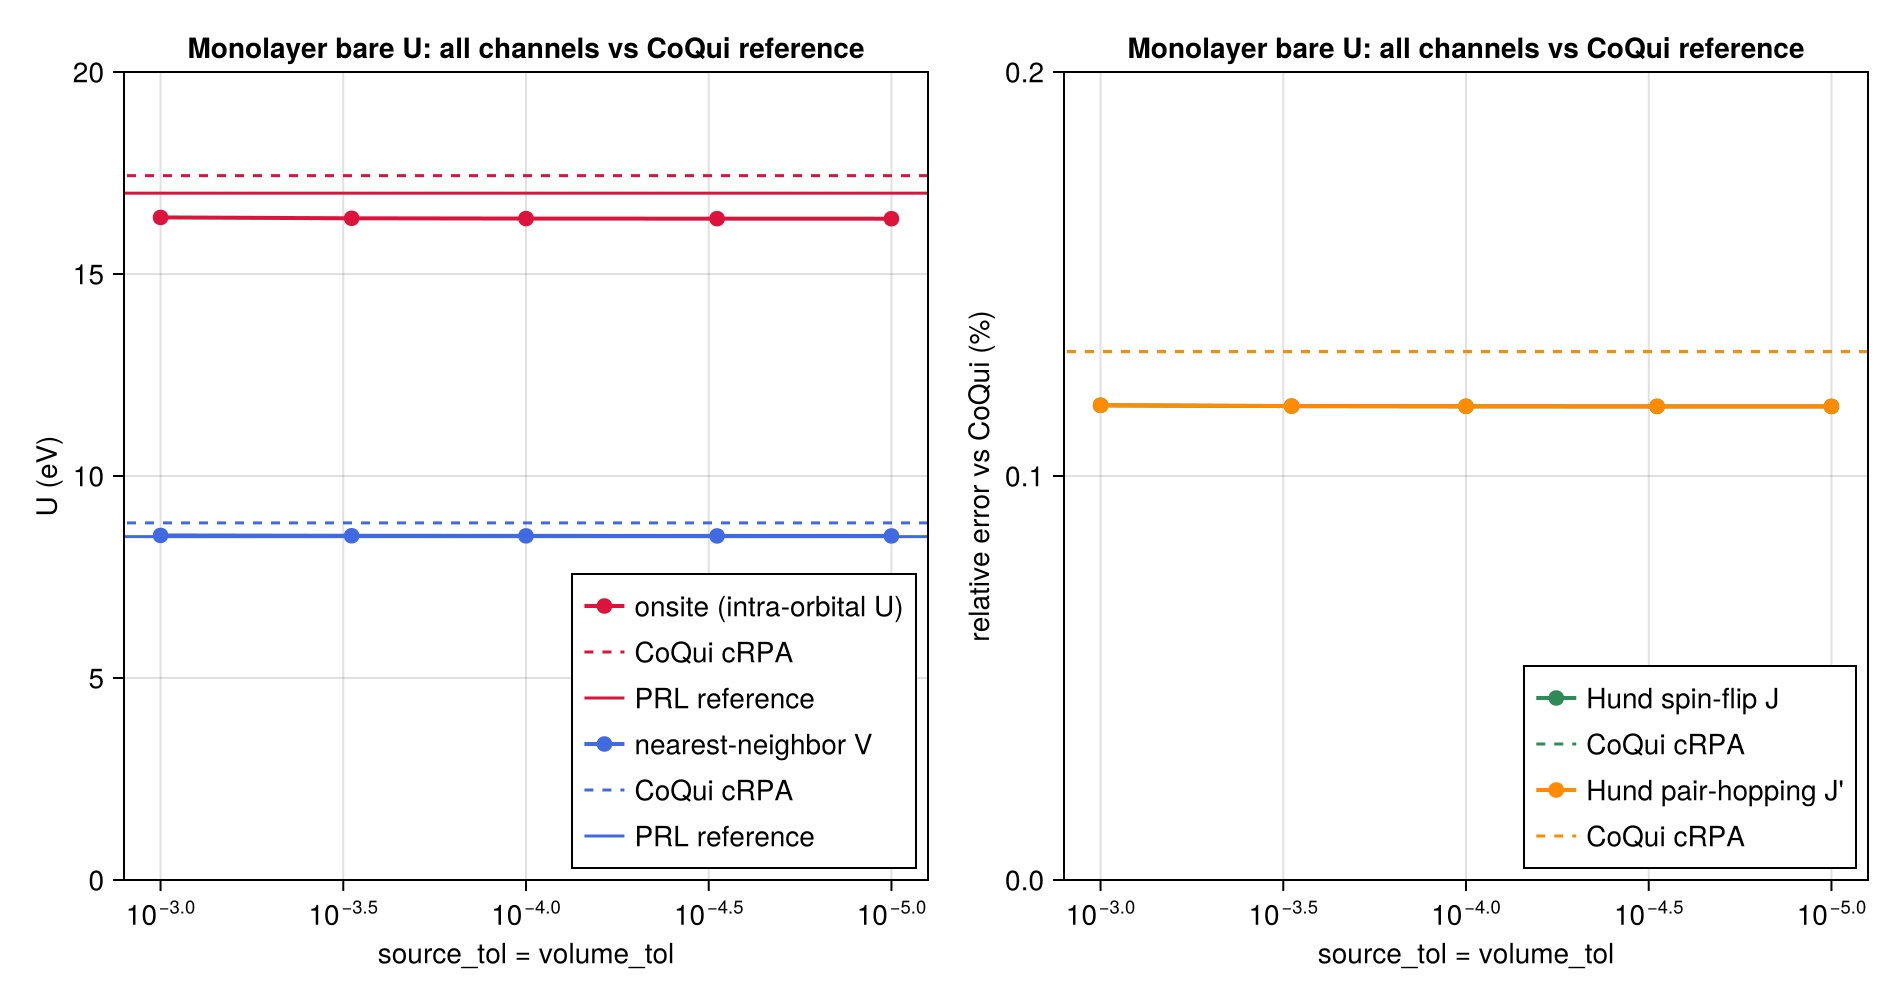
\includegraphics[width=0.85\linewidth]{../codes/graphene/figs/monolayer_tol_sweep_all_channels.png}
\caption{All four bare channels (onsite, NN, Hund's spin-flip, Hund's pair-hopping) versus quadrature tolerance. Dots are this work; dashed horizontal lines are the CoQui cRPA bare references; and solid lines are the PRL 106, 236805 values.}
\label{fig:tol_all}
\end{figure}

\begin{figure}[h]
\centering
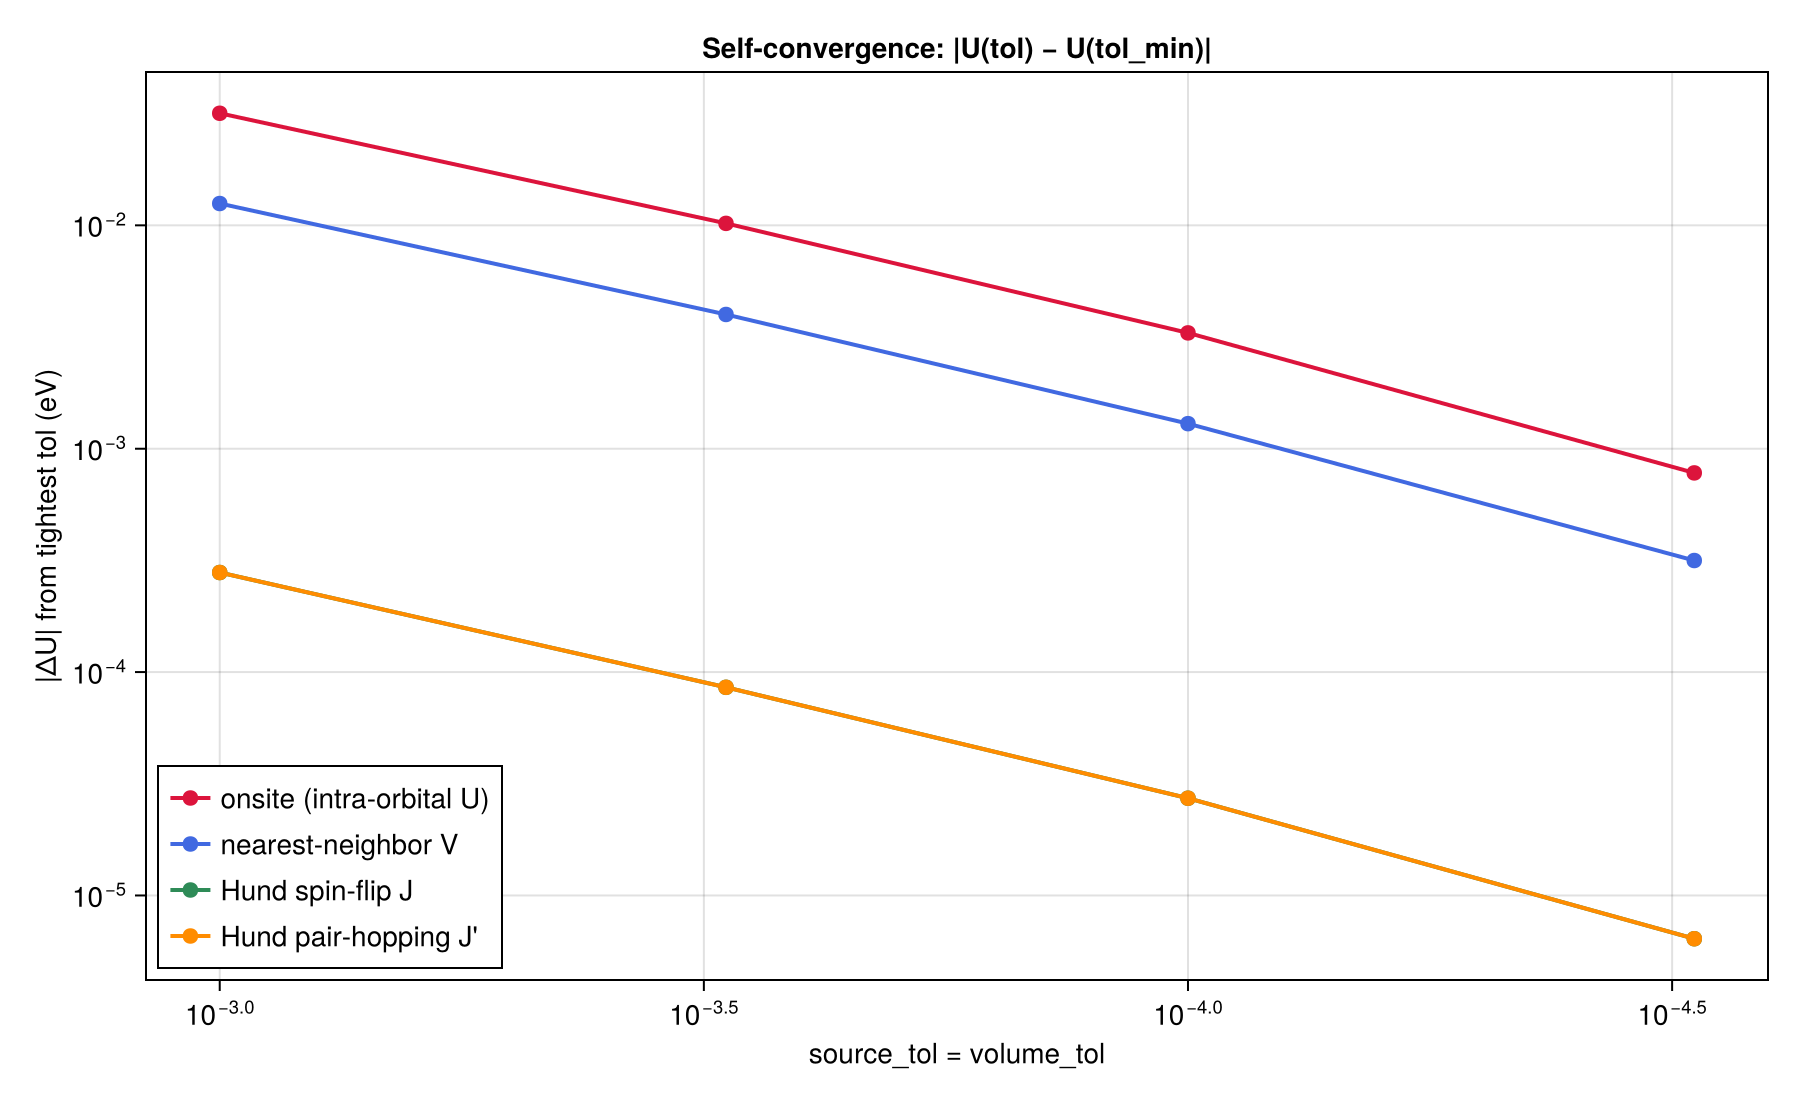
\includegraphics[width=0.85\linewidth]{../codes/graphene/figs/monolayer_tol_sweep_self_convergence.png}
\caption{Self-convergence of each channel: relative change of $U$ between successive tolerance levels. A clear convergence is observed, so the discrepancy with CoQui in Table 1 is not a quadrature error.}
\label{fig:tol_self}
\end{figure}

\newpage


\end{document}